\section{Анализ предметной области}

%Провести анализ предметной области технических текстов.
%Описать известные методы выделения составных частей научного текста.
%Сформулировать критерии сравнения описанных методов и провести их сравнительный анализ по выбранным критериям. 
 

\subsection{Структурный анализ документов}

Структурный анализ документов (Document layout analysis, DLA) --- процесс сегментирования входного изображения документа на однородные компоненты, такие как блоки текста, рисунки, таблицы, графики и т.д., и их соответствующей классификации~\cite{tnt}.

Процесс структурного анализа документов состоит из двух основных этапов --- предобработки и анализа структуры документа~\cite{dla-survey, dla-book}.

На рисунке ниже приведена схема процесса структурного анализа документов.

% TODO: Russia
\begin{figure}[H]
	\centering
	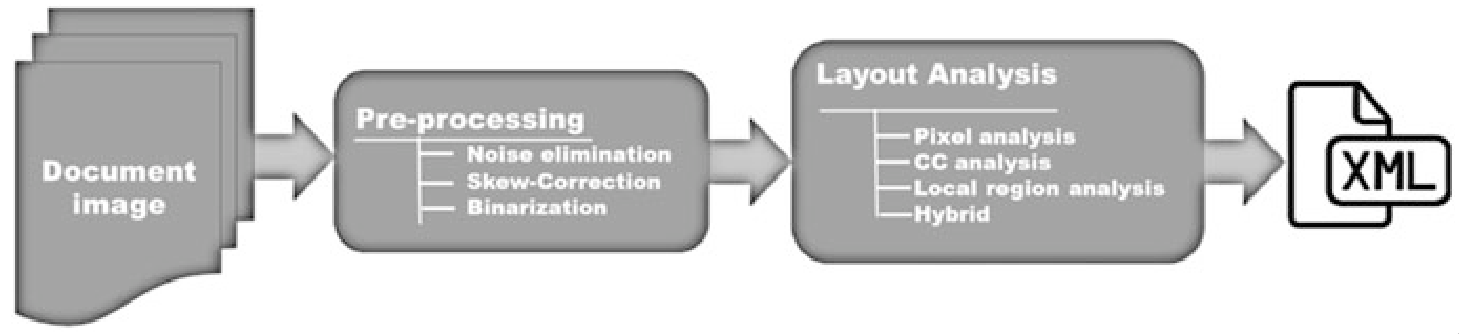
\includegraphics[width=\textwidth]{img/typical-dla-system.png}
	\caption{Схема процесса структурного анализа документов~\cite{dla-book}}
	\label{fig:}
\end{figure}

\subsubsection{Этап предобработки}

\subsubsection{Этап анализа структуры документа}

% Что такое DLA, зачем

% Какие есть виды макетов, двухколоночные и т.д.
% Какие используются в научных статьях

%\subsection{Научно-технический текст}
\subsection{Структура научно-технического текста}

% Какие составные части у научного текста

% Есть разные определения, но для рассмотрения методов выделения составных частей НТТ полезно определить его со структурной точки зрения

% Научно

%Структуру научного текста можно рассмо

\cite{butenko2022}

\begin{figure}[H]
	\centering
	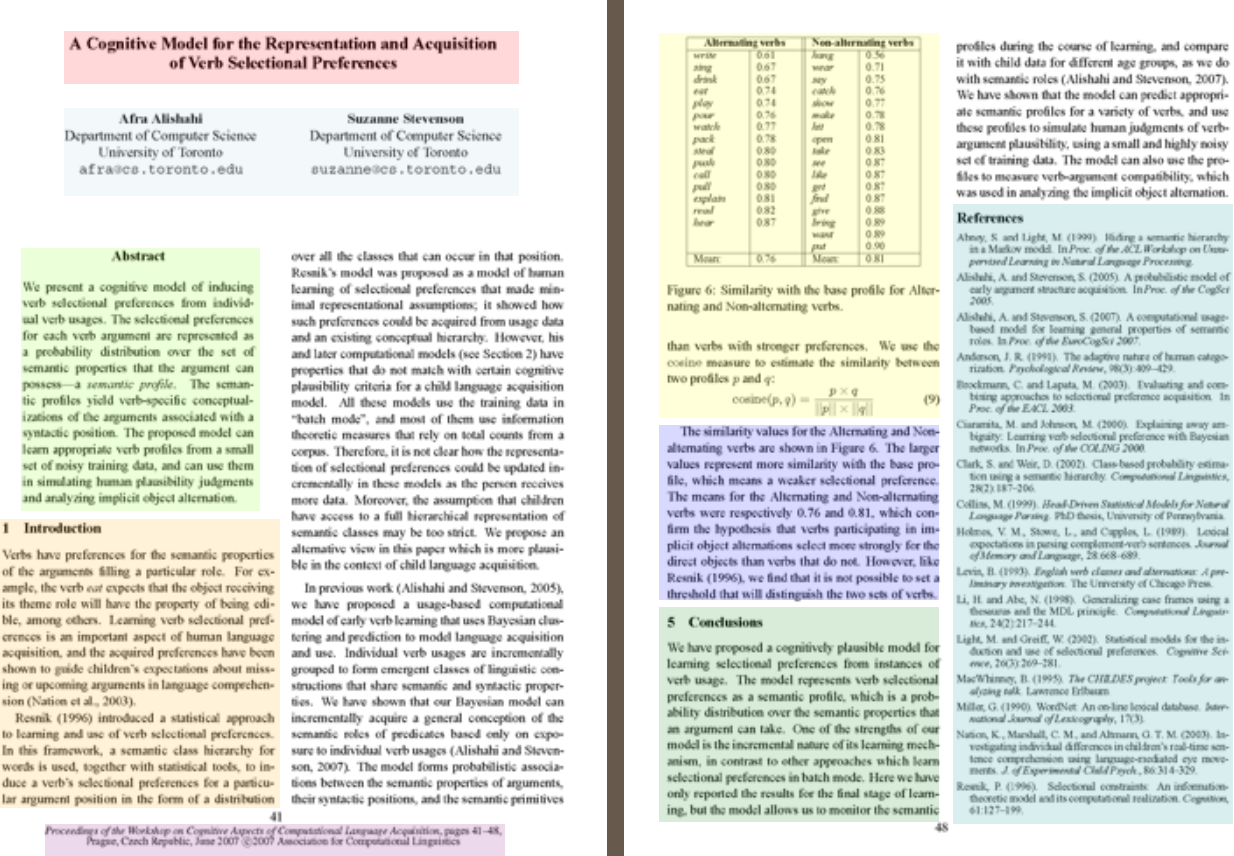
\includegraphics[width=\textwidth]{img/struct-parts.png}
	\caption{}
	\label{fig:}
\end{figure}

\begin{figure}[H]
	\centering
	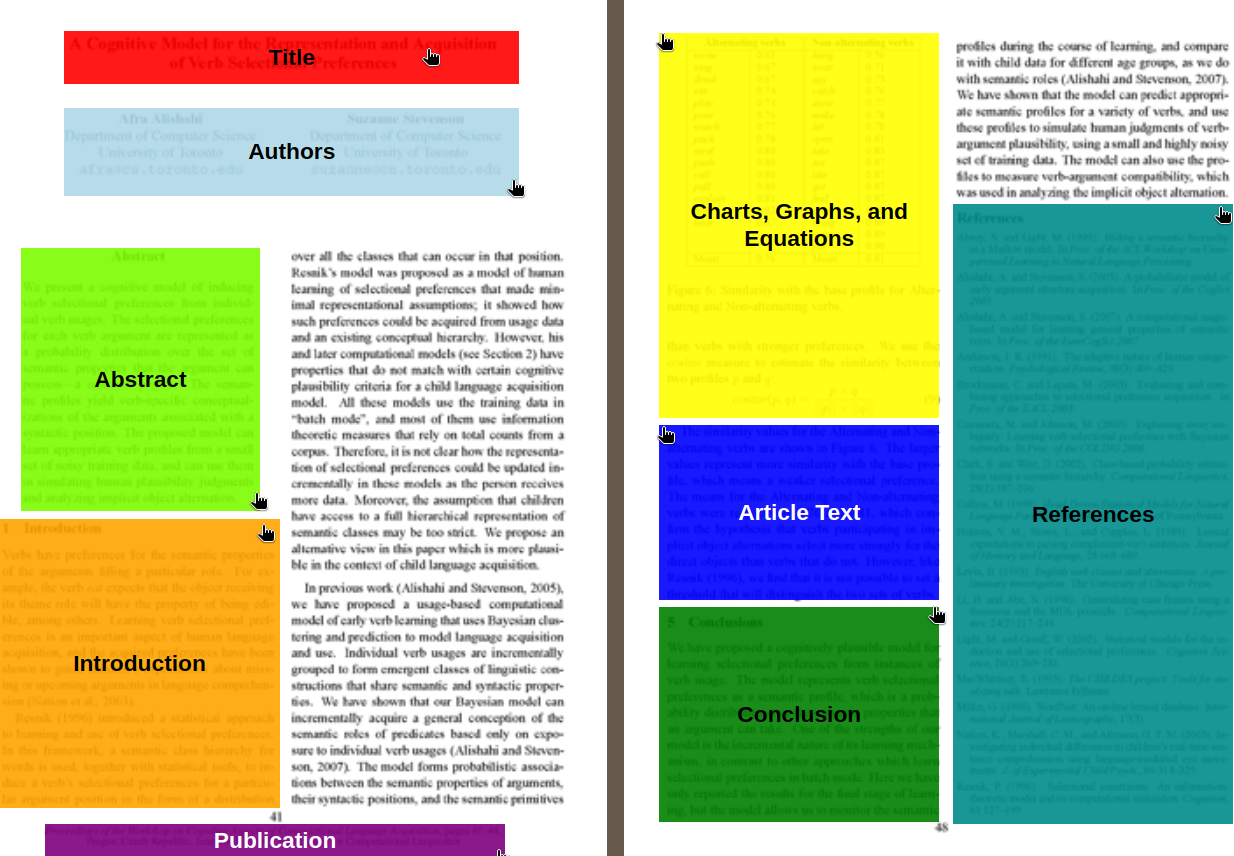
\includegraphics[width=\textwidth]{img/struct-parts-named.png}
	\caption{}
	\label{fig:}
\end{figure}

\section{Формализация задачи}

% Формализация, математическая

\section{Описание существующих методов}

% Куча методов

\subsection{Метод 1}

\subsubsection{Алгоритм 1}

\subsubsection{Алгоритм 2}

\subsection{Метод 2}

\subsubsection{Алгоритм 1}

\subsubsection{Алгоритм 2}

\subsection{Метод 3}

\subsubsection{Алгоритм 1}

\subsubsection{Алгоритм 2}

\section{Классификация существующих методов}

% Сформулировать критерии сравнения и сравнить; таблица
